% This file was created with tikzplotlib v0.10.1.
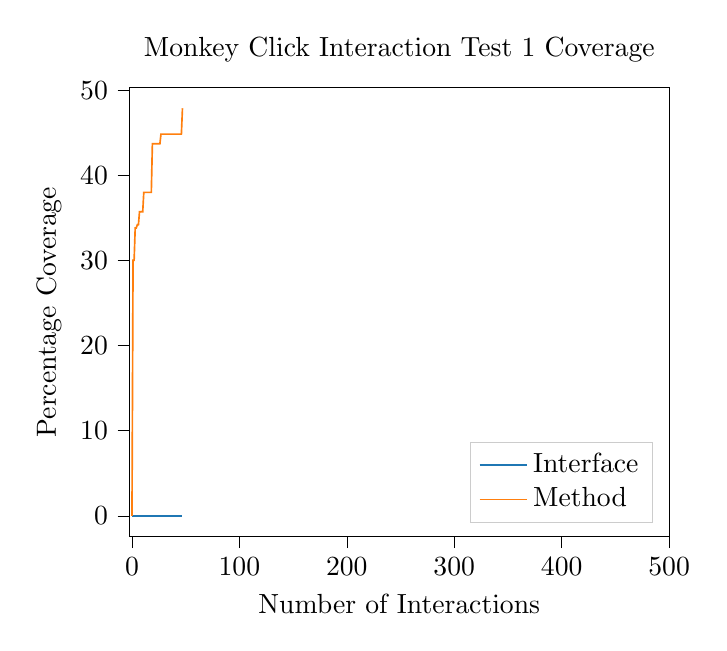
\begin{tikzpicture}

\definecolor{darkgray176}{RGB}{176,176,176}
\definecolor{darkorange25512714}{RGB}{255,127,14}
\definecolor{lightgray204}{RGB}{204,204,204}
\definecolor{steelblue31119180}{RGB}{31,119,180}

\begin{axis}[
legend cell align={left},
legend style={
  fill opacity=0.8,
  draw opacity=1,
  text opacity=1,
  at={(0.97,0.03)},
  anchor=south east,
  draw=lightgray204
},
tick align=outside,
tick pos=left,
title={Monkey Click Interaction Test 1 Coverage},
x grid style={darkgray176},
xlabel={Number of Interactions},
xmin=-2.35, xmax=500,
xtick style={color=black},
y grid style={darkgray176},
ylabel={Percentage Coverage},
ymin=-2.3955, ymax=50.3055,
ytick style={color=black}
]
\addplot [semithick, steelblue31119180]
table {%
0 0
1 0
2 0
3 0
4 0
5 0
6 0
7 0
8 0
9 0
10 0
11 0
12 0
13 0
14 0
15 0
16 0
17 0
18 0
19 0
20 0
21 0
22 0
23 0
24 0
25 0
26 0
27 0
28 0
29 0
30 0
31 0
32 0
33 0
34 0
35 0
36 0
37 0
38 0
39 0
40 0
41 0
42 0
43 0
44 0
45 0
46 0
47 0
};
\addlegendentry{Interface}
\addplot [semithick, darkorange25512714]
table {%
0 0
1 30.04
2 30.04
3 33.84
4 33.84
5 34.22
6 34.22
7 35.74
8 35.74
9 35.74
10 35.74
11 38.02
12 38.02
13 38.02
14 38.02
15 38.02
16 38.02
17 38.02
18 38.02
19 43.73
20 43.73
21 43.73
22 43.73
23 43.73
24 43.73
25 43.73
26 43.73
27 44.87
28 44.87
29 44.87
30 44.87
31 44.87
32 44.87
33 44.87
34 44.87
35 44.87
36 44.87
37 44.87
38 44.87
39 44.87
40 44.87
41 44.87
42 44.87
43 44.87
44 44.87
45 44.87
46 44.87
47 47.91
};
\addlegendentry{Method}
\end{axis}

\end{tikzpicture}
